\documentclass{mprop}
\usepackage{graphicx}
\usepackage{longtable}

% alternative font if you prefer
%\usepackage{times}

% for alternative page numbering use the following package
% and see documentation for commands
%\usepackage{fancyheadings}


% other potentially useful packages
%\uspackage{amssymb,amsmath}
%\usepackage{url}
%\usepackage{fancyvrb}
%\usepackage[final]{pdfpages}

\begin{document}

%%%%%%%%%%%%%%%%%%%%%%%%%%%%%%%%%%%%%%%%%%%%%%%%%%%%%%%%%%%%%%%%%%%
\title{Extending QUIC to Support Real-Time Applications}
\author{Vivian Band}
\date{\today}
\maketitle
%%%%%%%%%%%%%%%%%%%%%%%%%%%%%%%%%%%%%%%%%%%%%%%%%%%%%%%%%%%%%%%%%%%

%%%%%%%%%%%%%%%%%%%%%%%%%%%%%%%%%%%%%%%%%%%%%%%%%%%%%%%%%%%%%%%%%%%
\tableofcontents
\newpage
%%%%%%%%%%%%%%%%%%%%%%%%%%%%%%%%%%%%%%%%%%%%%%%%%%%%%%%%%%%%%%%%%%%

%%%%%%%%%%%%%%%%%%%%%%%%%%%%%%%%%%%%%%%%%%%%%%%%%%%%%%%%%%%%%%%%%%%
\section{Introduction}\label{intro}

%briefly explain the context of the project problem

Transport protocols are an essential component of networked communications; they determine a 
number of important characteristics of traffic sent over Internet Protocol (IP) \cite{IP-RFC}, 
such as reliability, timeliness, and aggression. Ossification of the wider Internet has been 
enforced by middleboxes interfering with unrecognised traffic types, leading to the two most 
widespread options being the two transport protocols which were standardised the earliest: User 
Datagram Protocol (UDP) \cite{UDP-RFC} and Transmission Control Protocol (TCP) \cite{TCP-RFC}. 

UDP's lightweight design was originally intended to allow unreliable, low-latency communication, 
however, this property has benefits which have become increasingly notable in recent years: the 
lack of in-built behaviours as a result of reliability guarantees, combined with widespread 
acceptance by middleboxes, makes UDP an appealing blank canvas for engineers to use as a base for 
constructing flexible and widely deployable new userspace transport protocols.

QUIC \cite{quic-transport-16} is a userspace transport protocol currently being developed by Google and the Internet Engineering Task Force (IETF) as an alternative to TCP. QUIC has three distinct advantages over most implementations of TCP: it is much easier to deploy and modify as a result of not requiring kernel modifications; both payload content and the majority of header fields are encrypted by default; and it uses multiplexed streams to avoid problems with head-of-line blocking. The protocol is still in the design stage, with the majority of development focused on the use-case of HTTP/2 \cite{HTTP2-RFC} web traffic with ordered content and relaxed latency bounds.

In this project, I aim to show that QUIC can be adapted for a significantly different use-case: 
real-time, interactive media using the Real-Time Transport Protocol (RTP) \cite{RTP-RFC} over 
QUIC. This version will improve on similar previous work, implementing deadline and dependency 
awareness in addition to selective restransmissions rather than solely discriminating based on 
media frame type (i.e. I-frames, P-frames) \cite {Palmer2018}.

%%%%%DISCARDED FRAGMENT, MIGHT BE USEFUL LATER%%%%%
%TCP has received much refinement in the 37 years since its initial standardisation, however, it 
%is becoming increasingly difficult to deploy the kernel-level changes needed for new 
%optimisations to take effect as the number of machines on the Internet continues to increase. 
%For example, TCP Fast-Open, a modification standardised in December 2014, is still not deployed 
%in a majority of Internet-connected devices as of early 2018 \cite{tfo-failures}.

The remainder of this report consists of the following sections:

\begin{itemize}
	\item \textbf{Section 2: Statement of Problem} explains the motivations for extending QUIC to 
	run RTP.
	\item \textbf{Section 3: Key Differences Between Underlying Transport Protocols for RTP} 
	details the key functional and semantic incompatibilities between stream-based transport 
	protocols and RTP.
	\item \textbf{Section 4: Literature Survey} explores previous attempts at running RTP over a 
	stream-based transport protocol.
	\item \textbf{Section 5: Proposed Approach} describes the deliverables of this project, how 
	they relate to the aims outlined in section 2, and the processes used to create them.
	\item \textbf{Section 6: Work Plan} provides a proposed schedule for the deliverables outlined 
	in section 5.
\end{itemize}

%\subsection{A subsection}
%Please note your proposal need not follow the included section headings - this is only a suggested structure. Also add subsections etc as required

%example references: \cite{BK08}

\newpage

%%%%%%%%%%%%%%%%%%%%%%%%%%%%%%%%%%%%%%%%%%%%%%%%%%%%%%%%%%%%%%%%%%%
\section{Statement of Problem}

%clearly state the problem to be addressed in your forthcoming project. Explain why it would be worthwhile to solve this problem.

QUIC is reported to serve up to 9.1\% of Internet traffic as of 2018, with 98\% of this being 
generated by Google services \cite {Ruth2018}. The IETF is still in the process of standardising 
the first version of the protocol, with the involvement of engineers from various high-profile 
technology companies, however, development is currently focused on improving the performance of 
HTTP.

QUIC offers reliable delivery of ordered data, only delivering data to 
applications when all packets up to the most recently received have been recovered and 
reassembled in the correct order. This behaviour results in increased latency and makes QUIC a 
poor choice as an underlying transport protocol for real-time, interactive applications like 
Voice over IP (VoIP) or multiplayer gaming, especially given that these applications are more 
adversely affected by high-latency than by packet loss. RTP over UDP is typically used for real-time applications; the lack of reliability or ordering guarantees in either protocol minimises latency at the expense of occasional packet loss and out-of-order delivery. This is a balance which generally provides the best quality of experience for real-time applications like the earlier examples of VoIP or multiplayer gaming: their primary concern is to respond to input from remote users in the shortest time possible, an aim which can be achieved even with some packet loss and unordered delivery.

The defining strength of userspace protocols is their flexibility: a version of QUIC 
which uses selective restransmissions and has awareness of deadlines could potentially outperform 
UDP in terms of quality of experience for real-time applications, as well as providing greater 
security through use of encrypted traffic. This project aims to create a set of extensions which 
allow QUIC endpoints to use partial reliability for interactive, real-time applications, most 
likely through sending transport parameters during initial connection setup.

\newpage


%%%%%%%%%%%%%%%%%%%%%%%%%%%%%%%%%%%%%%%%%%%%%%%%%%%%%%%%%%%%%%%%%%%
\section{Background and Rationale}

\subsection{Streaming using MPEG DASH}

Dynamic Adaptive Streaming over HTTP (DASH) is used by high-profile companies like Netflix to deliver media which does not does not have strict latency bounds, such as on-demand TV streaming. Chunks of media content, typically with a duration between 1 and 10 seconds \cite{Palmer2018}, are requested by the client from a manifest file as a series of HTTP \texttt{GET} requests, but HTTP generally uses TCP as an underlying transport protocol and DASH encounters problems with stalling due to head-of-line blocking within TCP as a result. An example of this is illustrated in Figure 1.

\begin{figure}[h]
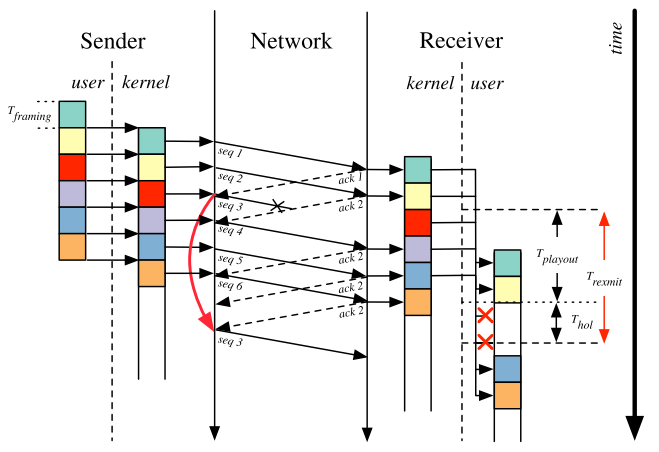
\includegraphics[scale=0.4]{images/holtcp}
\centering
\caption{Head-of-line blocking within TCP as illustrated by McQuistin \textit{et al} \cite{McQuistin2016}. The loss of the packet with sequence number 3 prevents any subsequent packets being delivered to the application until it is received.}
\end{figure}

QUIC mitigates this issue by using several streams demultiplexed 
over a single UDP socket. Although head-of-line blocking still occurs in response to loss, the 
obstruction is confined to a single stream rather than blocking the entire connection. With some 
adjustments to optimisation algorithms used in DASH, QUIC could be used to provide higher quality 
streaming services for unidirectional media content \cite{Bhat2017}.

While buffering can be a source of irritation to the end user, the content being generated and sent does not change based on their input and some delay can be tolerated. An application sending media using DASH closely resembles many other HTTP-based applications and is easier to implement for delay-tolerant media than an RTP equivalent, which requires more extensive configuration.

\subsection{Interactive Media using RTP}

Real-time, interactive media is commonly streamed using RTP over UDP. Applications using RTP prioritise low 
latency over reliability; the end-user experience of VoIP sessions and multiplayer games, for 
example, is significantly impacted by even minor delays in data reaching the application, but a 
small amount of packet loss can be concealed and out-of-order delivery can occasionally be 
corrected within RTP.

Although more complicated than DASH, where media is delivered as a series of \texttt{HTTP GET} 
requests, RTP allows applications to customise how data should be formatted and transferred 
between participants through the use of RTP profiles \cite{RTP-RFC}. This flexibility allows RTP 
to be used for a wide range of interactive applications, including technologies which have only started 
to become widespread in recent years such as virtual reality and augmented reality. QUIC's behaviours are similarly malleable due 
to not requiring any kernel modifications: while guaranteed reliability is not desirable for 
real-time applications, an extension to QUIC which introduces partial reliability alongside 
existing stream demultiplexing capabilities, framing, and increased security could be highly 
desirable for real-time, interactive media.

\subsection{Transport Protocols - Reliability vs Latency}

Reliable transport protocols like TCP and QUIC are not optimal choices for real-time, interactive 
applications like VoIP due to prioritising reliability over timeliness. Guaranteed reliability is 
useful for applications with relaxed latency bounds and strict ordering requirements (eg. serving 
web pages), but head-of-line blocking in response to packet loss impairs the performance of time-sensitive applications typically using RTP. This effect is noticeable even when the delay is confined to a single stream within a QUIC connection as it risks breaking synchronisation between different media channels (eg. mismatch between audio and video).

RTP over UDP typically achieves low-latency by not attempting to recover lost packets, opting to use feedback from RTCP sender and receiver reports to change the quality of media generated by the codec if a session experiences significant loss. However, a dropped packet could still be useful to the application, provided it can be retransmitted by the sender and processed by the receiver before the playback deadline. This functionality is known as partial reliability, which consists of selectively retransmitting frames that are deemed to meet the playback deadline under current network conditions, and dropping frames which exceed it. At least one of the transport protocols used needs to have deadline awareness, which requires a moving average of RTTs, current playback position, and timestamps of recently lost frames. This behaviour could be implemented within an intermediary layer or within the QUIC protocol.

Dependencies between frames also need to be considered: P-frames change visual information relative to a previously sent I-frame, so a `stale' I-frame which will not arrive at the application before the playback deadline may still need to be retransmitted to allow useful P-frames to work. Either QUIC or an intermediary layer needs to be aware of which QUIC packets contain specific I-frames and which P-frames rely on them for this behaviour to work. This is complicated further by the possibility that multiple QUIC packets may be required to accomodate a single I-frame, depending on the maximum packet size allowed.

A retransmission scheme for RTP has already been published as RFC 4588 \cite{RTP-retransmission-RFC}. While this document acknowledges the challenges of implementing deadline awareness, it also assumes that RTP will be running over UDP rather than a reliable, stream-oriented transport. Running RTP over QUIC does have the advantage of not needing to re-implement base acknowledgement and retransmission functions from scratch, but the reliable retransmission and buffering behaviours within QUIC will need modification for selective retransmission and deadline awareness to work. These alterations cannot be performed at an intermediary layer or within an RTP-based application, and will add more complexity to the QUIC specification.

In summary, a transport protocol for real-time media must prioritise timeliness over reliability and in-order delivery. This does not mean it should never retransmit packets, however; lost packets should be retransmitted if they are likely to reach the client application before their playback deadline, or if they are required by the application to process dependent frames which will meet their deadlines. Existing retransmission mechanisms within reliable transports like QUIC can be modified and awareness of deadlines introduced to selectively retransmit packets based on their potential usefulness.

\subsection{Real-time Transport over QUIC}

A key feature of QUIC traffic is that all content, including the majority of header fields, is 
encrypted by default using TLS 1.3 after completion of the cryptographic handshake 
\cite{quic-transport-16}. QUIC's focus on encrypted traffic as standard for increased security is 
likely to contribute towards an increased use of the protocol, combined with backing from 
influential technology companies and the ease of deploying userspace protocols.

Creating an RTP extension for QUIC is complicated by a semantic mismatch between the two protocols: RTP uses datagrams to transmit frame data and timing information, usually sending a single RTP frame per datagram, while QUIC is a stream-based protocol which does not have distinct boundaries between items of data once they are removed from their QUIC payload frames. It is not possible to guarantee a complete media frame will be extracted from the byte-stream due to not knowing its exact length - retrieving and parsing segments of arbitrary size to determine if one or more complete frames are present would add needless complexity to an RTP-QUIC extension, especially since a new parser would need to be written for each codec type.

An endpoint using QUIC over an IP link will aim to have a QUIC packet size between 1472 and 1200 bytes to avoid fragmentation at the IP layer \cite{quic-transport-16}. Predictive frames and bidirectional frames, known as P-frames and B-frames, only contain information about changes within an existing image and can be transmitted within a single QUIC packet without fragmentation due to their small size. Intra-frames, known as I-frames, are typically much larger because they contain information about an entire image and will need to be split over multiple QUIC packets. The payloads from packets containing I-frames will either need to be reassembled within QUIC and passed to the application as a single, complete frame, reassembled within the application itself, or reassembled within an intermediary layer.

\begin{figure}[h]
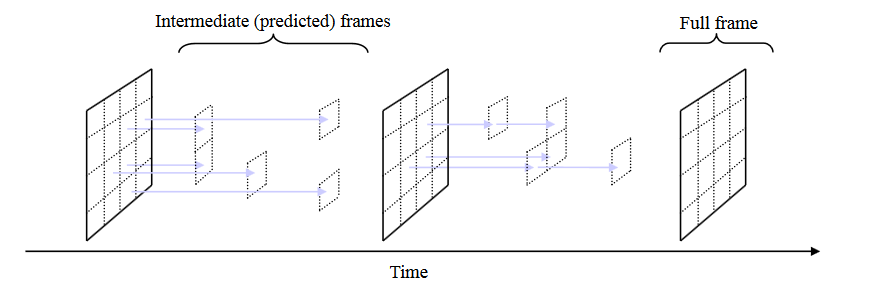
\includegraphics[scale=0.4]{images/iframepframe}
\centering
\caption{Relationship between I-frames and P-frames as illustrated by Perkins \cite{frame-diagram}. P-frames only change a section of an image previously described by an I-frame, reducing the amount of data which has to be sent by multimedia applications.}
\end{figure}

While reassembling I-frames entirely within QUIC makes the extension easier to use for developers of applications using RTP, it does also add complexity to an already extensive specification, requiring QUIC developers to add even more features to their implementations of the protocol. Reassembling I-frames within the application minimises the changes required to QUIC, but requires additional effort from developers working with real-time applications. The third option of offering a pre-built intermediary layer to handle RTP frame reassembly and error correction is a minimally invasive compromise for both parties, requiring no significant additions to QUIC and placing fewer technical demands on developers who wish to use the extensions, however, QUIC and the application using the extension have no requirement to validate that this layer is active on both endpoints. Similar considerations need to be made with regards to error correction for RTP frames: error correction and reassembly do not have to take place in the same locations, but it would likely be more sensible to perform error correction after reassembly since flaws could be missed while fragments are separated.

Application data units (ADUs) were first described by Clark and Tennenhouse as the smallest unit of data which an application can process out of order \cite{Clark1990}. Allowing the application to define the placement of frame boundaries is known as application level framing; these boundaries must be preserved by the underlying layers, including the transport layer, in order for ADUs to still be useful at the receiver. Real-time multimedia applications use frames as discrete units of data, but concatenating received frames into the byte-stream used within standard implementations of QUIC does not preserve the boundaries between frames. A message-based abstraction will be required in place of a byte-stream to ensure that frames remain independently decodable by the application.

\subsection{Conclusions}

The disparities between RTP and QUIC in terms of semantics and reliability make creating an RTP extension to the protocol challenging, however, QUIC's existing flow control mechanisms and emphasis on security as a default make it an appealing choice for transmitting real-time data. The flexibility of QUIC as a userspace protocol means it is possible to build a partially reliable, low-latency variant of QUIC suited to interactive media through use of selective retransmissions guided by deadline awareness. The byte-stream used within QUIC by default needs to be replaced with a message-oriented abstraction to allow applications to process units of data independently of each other, allowing out-of-order delivery to occur within the transport.

\newpage

%%%%%%%%%%%%%%%%%%%%%%%%%%%%%%%%%%%%%%%%%%%%%%%%%%%%%%%%%%%%%%%%%%%
\section{Literature Survey}

%present an overview of relevant previous work including articles, books, and existing software products. Critically evaluate the strengths and weaknesses of the previous work.

Although QUIC is still in the process of IETF standardisation, there is academic interest in extending the protocol. The EPIQ workshop \cite{epiq}, hosted as part of ACM CoNEXT 2018, featured two papers which are directly relevant to this project: a discussion of the challenges of supporting real-time media in QUIC and a proposed set of extensions, QUIC-R, by Perkins and Ott \cite{Perkins2018}; and ClipStream, a version of QUIC featuring partially reliable streams by Palmer \textit{et al} \cite{Palmer2018}.

There are several key themes which emerge from previous work on optimising existing transport protocols for real-time, interactive applications. The most important of these is the effects of latency: while applications with relaxed latency bounds, such as on-demand video streaming, can tolerate delay and benefit from reliability and ordering, the primary aim of real-time, interactive applications is to appear to respond to user input instantaneously at the expense of a slight reduction in playback quality. This need for low-latency over reliability naturally leads into discussion of the reliability provided by the underlying transport, and under what conditions it should be modified; providing selective reliability based on whether content will arrive at the receiver in time to be useful is a sensible approach, but potentially complicated to implement when considering frame dependencies. Application data units are considered in order to eliminate dependencies at the decoding stage of receiving media content, and to allow data to be independently usable to applications to the greatest extent possible. Comparisons between the two most widely deployed transport protocols, UDP and TCP, as substrates for a media-aware transport are considered, before finally reviewing material suggesting how such a transport could be implemented within QUIC.

\subsection{Use-Cases for DASH and RTP}

The QUIC-R paper presented at EPIQ by Perkins and Ott contains valuable background information about the evolution of video streaming technologies and their potential place in QUIC. RTP was historically used to stream media on less reliable networks from the mid-1990s, but applications using this protocol are complex due to the mechanisms required to mitigate the effects of packet loss and out-of-order arrival. DASH is less complex, providing media content in pre-encoded chunks through a series of HTTP \texttt{GET} requests; this approach has become more widely used as networks have increased in quality and demand has risen for unidirectional streaming (i.e. the content being sent is not impacted by the actions of the receiver and therefore has more relaxed latency bounds). RTP remains the best option for interactive, real-time media where timeliness is a priority, and for streaming over less reliable networks.

\subsection{Mapping RTP onto TCP}

Adapting a mapping of RTP onto TCP specified in RFC 4751 \cite{RTP-TCP-RFC} for use with QUIC is discussed, but deemed unacceptable for applications with strict latency bounds. This is due to problems with head-of-line blocking which are inherent in all standard TCP stacks: any packets received by a TCP socket with a sequence number greater than the one held by a lost packet cannot be accessed by the application until this lost packet is received. Even if content flows can be multiplexed within the application, all flows are blocked by instances of packet loss even for streams unrelated to the content within the lost packet. An individual stream within QUIC does not suffer head-of-line blocking due to loss on other streams within the connection due to streams being multiplexed over a UDP socket, but it does still encounter high latency due to loss within its own stream. This is a problem for real-time multimedia applications where content delivered on parallel streams may be require synchronisation, such as lip-synchronisation on video calls.

\subsection{Reliable and Unreliable QUIC Streams}

The idea of marking some QUIC streams as either reliable, partially reliable, or unreliable was proposed in an IETF draft by Tiesel \textit{et al} \cite{Tiesel2017}. A separate draft by Lubashev \cite{Lubashev2018} elaborates on partial reliability and message abstractions within QUIC, using single octet gaps to notify the application of message boundaries and marking data written to the transport as transmittable or non-retransmittable using offset markers. This approach may work for real-time media through marking data sent before the most recently sent I-frame as being ineligible for retransmission, but this does not guarantee that retransmitted frames will arrive before their respective playback deadlines. I-frames could be sent at an increased frequency to minimise this issue, but this would impact performance due to applications having to process a large amount of image data more frequently as well as potentially having to retransmit larger frames more often.

An approach which is less generalised, but does not require extensive configuration at the application level is explored in a paper by Palmer \textit{et al} \cite{Palmer2018}, which was presented as part of the EPIQ workshop alongside the background analysis work by Perkins and Ott. Their extensions to QUIC, named ClipStream, sends I-frames and end-of-stream markers reliably, while P-frames and B-frames are sent on unreliable streams. These unreliable streams perform opportunistic transmission, sending new data instead of retransmitting lost data. This is an improvement on marking contiguous sections of data as retransmittable or non-retransmittable due to less non-useful data being retransmitted, but it assumes that resending P-frames and B-frames is always unnecessary; retransmitting these frames if they will arrive before the playback deadline would improve media quality with no significant disadvantages.

ClipStream requires an application to specify which type of stream it wants to use for sending video files, but the underlying complexities of video reassembly and reliability are abstracted away in several shim layers and 200 lines of modification to the chosen QUIC implementation, \texttt{quic-go}. A reliable control stream containing multiplexing and demultiplexing information to co-ordinate the reads of QUIC streams performed by the receiver, allowing it to reconstruct the sent video file. It also uses a shim layer at the sender to mark I-frames as reliable and P-frames and B-frames as unreliable, and another shim layer at the receiver to reassemble the video frames in the correct order before passing this data to the client application.

\subsection{Deadline Awareness}

The API required to use ClipStream is simple compared to the partially reliable streams described by Tiesel and Lubashev, but all three of these approaches lack awareness of playback deadlines for real-time media. This is less of an issue for media playback where latency bounds are more relaxed, such as on-demand TV streaming services, but for applications which should appear to respond to user interactions in real-time, such as multiplayer gaming or video conferencing, determining the usefulness of content before (re-)sending is vital for reducing the amount of unnecessary data sent, and therefore reducing latency as much as possible. Creating a shim layer to calculate estimated arrival times and projected playback deadlines is more complex than simply marking frames as reliable or unreliable, as happens in ClipStream, but would improve video quality as perceived by end-users; the number of stalls is likely to be similarly low, given that I-frames are retransmitted if needed, but movement within the video should appear to be smoother if useful P-frames are also retransmitted.

Previous attempts have been made to implement deadline awarness for partial reliability within reliable, byte-stream oriented transports. TCP Hollywood, a transport protocol developed by McQuistin \textit{et al} \cite{McQuistin2016} for use with real-time applications, has awareness of playback deadlines for real-time applications to determine the usefulness of retransmittable content. If a message marked for retransmission will not reach the receiver before its associated playback deadline, TCP Hollywood will send a different message which will be useful under the same TCP sequence number instead. These are known as inconsistent retransmissions, and are analagous to placing different data into a retransmitted \texttt{STREAM} frame in QUIC; ClipStream performs a similar process, calling it `opportunistic transmission'. As of draft 16, QUIC endpoints may treat this as a \texttt{PROTOCOL\_VIOLATION} error and respond with a \texttt{CONNECTION\_CLOSE} frame \cite{quic-transport-16}, however, it is currently not mandatory. Inconsistent retransmissions could be used as an optimisation for real-time applications using QUIC, with the caveat that not all implementations of the protocol are required to accept this behaviour.

\subsection{Application Data Units}

TCP Hollywood delivers data to applications as independently decodable application data units through the use of a message-based abstraction instead of a byte-stream with no clear message boundaries. This removes the need for all data to be delivered to the appliation in-order: although P-frames and B-frames depend upon I-frames, I-frames can be used independently, and P-frames and B-frames can be used independently of each other. TCP Hollywood uses one leading and one trailing zero byte to mark each message, but data within QUIC is already enclosed within \texttt{STREAM} frames. Passing P-frames and B-frames to an application is relatively simple, given that they can be sent within a single \texttt{STREAM} frame in their entirety, but I-frames will be fragmented across several QUIC packets and will need to be reassembled into a single message; using new QUIC frame types to specify which type of video frame is being sent may assist in simplifying this process.

\subsection{UDP and TCP as Substrates}

McQuistin \textit{et al} note that they chose TCP as a substrate for their protocol over UDP due to the former being more commonly deployed in enterprise networks. A lack of access for UDP-based userspace protocols could potentially limit the deployability of real-time applications which use QUIC, but further work by McQuistin and Perkins states that repurposing UDP as a demultiplexing layer for userspace protocols is a good choice in the long-term \cite{McQuistin2016Ossification}; as userspace protocols gain traction as a result of backing by high-profile companies, such as Google in the case of QUIC, it is entirely feasible that an increasing number of enterprise networks will permit UDP traffic.

TCP Hollywood resists interference from middleboxes through being consistent with the wire-image of regular TCP, however, connections on cellular networks did not successfully deliver inconsistent retransmissions due to middleboxes interpreting the modified TCP packet payloads as data injection attacks \cite{McQuistin2016Ossification}. UDP, the substrate used for QUIC, is less likely to encounter issues with rejection and modification by middleboxes due to having less complex behaviour than TCP. QUIC traffic is particularly resistant to interference due to entire packets, with the exception of some header fields, being encrypted after completion of the cryptographic handshake; this allows QUIC to use inconsistent retransmissions on both cellular and fixed-line networks without interference from middleboxes.

As outlined in section 3, it is easier to modify behaviours in QUIC than TCP due to the former not requiring the authoring or distribution of kernel-level modifications. QUIC also suffers less from traffic being rejected or otherwise modified by middleboxes due to packets sent after completion of the cryptographic handshake being almost entirely encrypted: only a few header fields remain visible as plaintext to determine QUIC header type and which scheme should be used for decryption. Using a similar approach to TCP Hollywood in terms of deadline awareness and selective retransmissions would be beneficial to this project, however, it should not be blindly copied: in contrast to an assertion made by Perkins and Ott \cite{Perkins2018}, a study by Bhat \textit{et al} \cite{Bhat2017} showing degraded performance of DASH over QUIC compared to DASH over TCP suggests that extending the capabilities of QUIC is not as simple as directly replicating existing techniques seen in TCP.

\subsection{Proposed Deadline-Aware Extensions to QUIC}

Suggestions for implementing optimisations for real-time media in QUIC are given by Perkins and Ott in the form of a ``straw man proposal'' for a minimal set of extensions to the protocol, named QUIC-R. These extensions involve creating a new frame type, \texttt{RT\_STREAM}, to mark a stream as being used for real-time, interactive content with strict low-latency bounds. These RT-streams allow QUIC to use independently decodable application data units through sending records instead of holding data as a stream of bytes, the benefits of which are described in section 4.5. \texttt{RT\_STREAM} frame headers can optionally contain offset and length fields with the same meaning as regular \texttt{STREAM} frames, and must contain a sequence number for records and a timestamp in order for deadline awareness features to work. A field containing the minimum record sequence number to be retransmitted is also included in the header to allow for partial reliability; like the retransmission markers described by Lubashev \cite{Lubashev2018}, this minimum number field marks a contiguous section of the retransmission buffers within QUIC as containing stale data which should be removed, but this approach is different in that records which have a sequence number which exceed this minimum are not guaranteed to be retransmitted if their predicted arrival is later found to exceed the associated playback deadline.

A sender using QUIC-R writes a timestamp, a playback deadline, and any sequence numbers of previous records on which the current record depends; this will commonly be P-frames specifying which I-frame they reference. Timestamps are sent as part of the transmitted frame since they are required by receivers of applications using RTP, but playback deadlines and dependencies are held only at the sender to determine if a frame should be retransmitted; retransmissions will occur if a frame will be processed by the receiver before its playback deadline, or if other frames which are dependent on it will be processed by the receiver before their deadlines.

The receiver acknowledges packets in a similar manner to reliable QUIC, with the addition of sending an \texttt{ACK-Timing} frame to allow the sender to track RTT information for deadline awareness. The role of the receiver is primarily to pass frames and associated metadata to the application; real-time applications use timestamps and sequence numbers to reconstruct the timing and order of frames respectively. Playout buffering, synchronisation between media streams, and advanced error correction and concealment features are also left to the application layer to minimise the degree of modification required to the QUIC specification.

As explained in section 4.5, I-frames are large enough that they will need to be split across multiple QUIC packets and reassembled into a video frame before being delivered to the application. P-frames and B-frames are small enough that they will always be given to the application atomically, if at all, but question of how to handle a partially delivered I-frame is left to the application layer; RTP payload formats should specify which course of action to take in the event of receiving an incomplete frame. This project will follow a similar approach and defer the handling of incomplete frames to the application layer for the time being.

\subsection{Summary}

The API required by real-time QUIC extensions similar to QUIC-R will likely be quite simple, unlike the APIs required for the approaches suggested by Tiesel and Lubashev; applications will make calls to send and receive messages containing a media frame from a QUIC socket in a similar manner to TCP Hollywood sockets. The partially reliable retransmission strategy based around deadline awareness will also be similar to TCP Hollywood, with frames being retransmitted if they will meet their playback deadline or if their retransmission is required to allow dependent frames to meet their playback deadlines.

A field containing the minimum retransmittable message sequence number as suggested for QUIC-R will be used to ensure the retransmission buffers within QUIC are kept clear of frames which have not been acknowledged but will never be retransmitted, either due to their own playback deadlines expiring or the deadlines of all of their dependent frames. Unlike ClipStream, the extensions in this project will send all data over partially reliable streams, but sending QUIC frames required to close streams reliably within these streams is essential to avoid `zombie' streams, as described in the draft by Tiesel.

\newpage

%%%%%%%%%%%%%%%%%%%%%%%%%%%%%%%%%%%%%%%%%%%%%%%%%%%%%%%%%%%%%%%%%%%
\section{Proposed Approach}

%state how you propose to solve the software development problem. Show that your proposed approach is feasible, but identify any risks.

\subsection{Priority Assessment}

The required, potential, and discounted additions to QUIC and shim layers for this project are as follows:

\begin{longtable}{|p{3.5cm}|l|p{8.5cm}|} 
\hline
Section & Importance & Reasoning \\ \hline
Message-oriented abstraction  & Must have & The concept of application data units is important to minimise the number of dependencies where possible: individual frames may require another frame to be useful in media playback, but the application should be able to decode them independently of each other. An application should be able to read individual, meaningful messages instead of attempting to parse (potentially incomplete or corrupt) frames from a raw byte-stream. This requirement also involves attempting to reassemble I-frames which must be split across several QUIC packets into a single message. \\ \hline
Partial reliability & Must have & Required to eliminate latency caused by head-of-line blocking. Also allows the retransmission of useful and/or important frames and the dropping of frames without dependencies which will not arrive before their associated deadline. \\ \hline
Deadline awareness & Must have & Required to decide which frames should be retransmitted based on whether their dependencies and playback deadlines. Will improve the quality of media playback by enabling the retransmission of video frames regardless of their type. \\ \hline
API & Must have & Required to allow for testing. A simple API would be preferred to make the extensions easy to use. \\ \hline
Testbed & Must have & A controlled environment for testing is essential to evaluate the effectiveness of the new extensions. \\ \hline
Dependency information & Should have & `Stale' I-frames which will not meet a playback deadline by themselves but have dependent frames which will meet their deadlines need to be retransmitted. \\ \hline
Inconsistent retransmissions & Could have & Could increase the efficiency of sending new material, but could also cause problems with some QUIC implementations if they decide to treat inconsistent payloads as a protocol error. \\ \hline
Frame re-ordering and timing & Could have & The QUIC-R extensions paper suggests leaving this to the application layer, but ClipStream uses a shim layer to reconstruct video files through co-ordinating reads from QUIC streams. It may be possible to implement this as a separate shim layer if time permits. \\ \hline
Forward error correction & Won't have & Highly unlikely to be implemented within the given time constraints due to complexity. \\ \hline
Multiple participants & Won't have & QUIC-based applications are currently limited to two participants due to the protocol being connection-oriented. Developing a multi-party, interactive application would require implementing peer-to-peer features within QUIC, which is not feasible within the time permitted.\\
\caption{MoSCoW priority assessment for real-time extensions to the QUIC protocol.}
\label{priority-assessment}
\end{longtable}

\subsection{Deliverables}

The first step in the development process is to write a simple application in C which creates RTP packets and sends them to a remote peer over UDP; these packets will be correctly formatted in terms of headers, but they will not send meaningful media content. This will initially be written as a unidirectional application, and will then be modified to send data and RTCP info from both participants simultaneously. This will require three threads: one for sending data and RTCP reports, one polling the UDP socket for new RTP data and RTCP feedback, and one processing received data and reports. After this, the application will be modified to send correctly encoded media data using the H.264 codec; the video used will be the open-source \textit{Big Buck Bunny}.

The next stage is to change the underlying transport from UDP to QUIC, initially using a single standard, reliable QUIC stream for all media content and a separate stream for RTCP operations, all of which will be sent using standard \texttt{STREAM} frames. The performance will be suboptimal and TCP-like due to head-of-line blocking, but this is a necessary step to become familiar with the chosen QUIC implementation. The project will use \texttt{ngtcp2} because it is compliant with a recent draft of the QUIC specification (draft-15 at the time of writing \cite{quic-implementations}); it is written in a familiar language, C; and it features the full range of client, server, and library roles. Alternatives which meet similar criteria such as \texttt{f5}, \texttt{picoquic}, \texttt{quant} are available if any unforseen problems occur with \texttt{ngtcp2}.

The loss recovery mechanisms within chosen implementation of QUIC will then be modified to support partial reliability, testing on a minimal two-stream application with 10\% of QUIC packets scheduled to be dropped using \texttt{netem}; if packets which are not received by participant B are no longer queued at participant A, then the default guaranteed loss recovery behaviour has successfully been modified. This will be unidirectional at first to simplify testing and debugging, and will then progress to bidirectional streams.

Deadline awareness will then be developed for the application using timestamps, message sequence numbers, and playback deadlines. The receiver will need to send a receipt of which messages arrived at which time; these will be used as part of a moving average to calculate current round-trip times (RTTs) to predict the usefulness of future media frames, but are not needed to remove packets from the retransmit queue as this is already handled by regular ACKs within QUIC. After each ACK, a new lowest retransmittable sequence number will be calculated based on average RTT calculated using a range of the most recent message receipts (eg. the last 10 observed RTTs); all frames with a sequence number lower than this will be removed from the retransmit queue if they have no dependent frames which are equal to or exceed this number. Using a moving average of several values for estimated RTT will mitigate the effect of isolated delay spikes removing large amounts of data from the retransmit buffer which could still be useful later when the next RTT returns to previous lower values. The logic for calculating deadlines and usefulness will likely be in a shim layer between QUIC and the application to begin with, but may be moved within QUIC if the modifications required are not too substantial. Retransmission of packets which remain within the retransmit buffer will be performed using standard QUIC mechanisms.

After partial reliability, deadline awareness, and frame dependencies have been implemented successfully, a testbed will be designed for evaluation. This will be created using Mininet \cite{mininet}, a virtual network which can be configured as required for testing under controlled conditions. Considerable thought needs to be given to designing this environment, so two weeks will be allocated for designing and writing management scripts to automate experiments as far as possible.

Tests will be run on this virtual network to gather data based on the playback of \textit{Big Buck Bunny}, encoded using FFmpeg \cite{ffmpeg} at a frame rate of 24 frames per second. The metrics to be measured are the buffering ratio, which is the ratio of time spent buffering to the total video duration, and the buffering rate, which is the rate at which stalls occur in terms of the total number of video frames; these are deliberately similar to the metrics used by Palmer \textit{et al} to test ClipStream \cite{Palmer2018} in the interests of directly comparing the effectiveness of this project to previous work.

The number of chunks, which are an I-frame followed by a number of P-frames, carried by an individual stream created within the QUIC connection will be varied between 1 and N, where 1 is a new stream for each chunk and N is the total number of chunks in the video, in an environment with no loss to establish the optimal number of streams for delivering video content. Once this has been established, the percentage of loss introduced on the connection will be varied to observe how the QUIC extensions cope with adverse network conditions.

The final paper will be written once this data has been gathered, a process which is likely to take two to three weeks.

\newpage

%%%%%%%%%%%%%%%%%%%%%%%%%%%%%%%%%%%%%%%%%%%%%%%%%%%%%%%%%%%%%%%%%%%
\section{Work Plan}

%show how you plan to organize your work, identifying intermediate deliverables and dates.

\begin{itemize}
  \item January 2nd: Implement simple application in C which sends RTP packets containing dummy 
  data to peer.
  \item January 7th: Modify the application to send valid media data using H.264 codec.
  \item January 14th: Change underlying transport in application from UDP to QUIC, try to get all 
  content sent on a single stream initially.
  \item January 21st: Implement partial reliability by changing loss recovery and retransmission 
  behaviours within QUIC, test with 10\% packet loss in unidirectional traffic on localhost to 
  verify it works.
  \item February 4th: Create deadline awareness using a moving average in the shim layer tracking 
  the last 10 or so RTTs. Remove packets containing stale frames from retransmission buffers.
  \item February 18th: Improve deadline awareness to take frame dependencies into account - QUIC 
  packets containing a stale I-frame should still be retransmitted if there are live P-frames 
  which depend on it.
  \item February 25th: Design of Mininet environment and testing scripts.
  \item March 11th: Testing different numbers of chunks to be sent on each stream.
  \item March 18th: Testing different amounts of loss on the connection.
  \item March 25th: Write paper.
\end{itemize}

\begin{figure}[h]
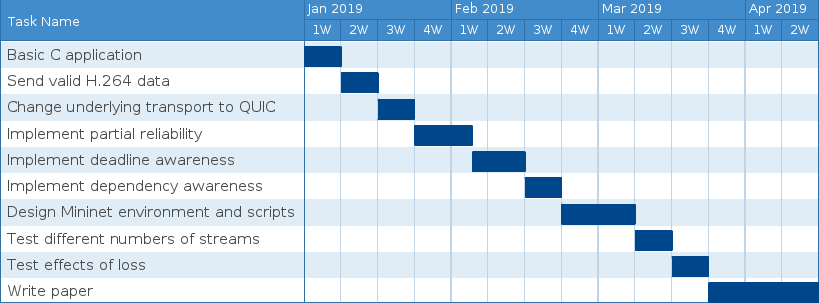
\includegraphics[scale=0.5]{images/gantt}
\centering
\caption{Gantt chart of proposed development timeline}
\end{figure}

\newpage

%%%%%%%%%%%%%%%%%%%%%%%%%%%%%%%%%%%%%%%%%%%%%%%%%%%%%%%%%%%%%%%%%%%
% it is fine to change the bibliography style if you want
\bibliographystyle{plain}
\bibliography{mprop}
\end{document}
